\section{Subgrafos}
\label{sec:subgrafos}

\begin{definicion}{Subgrafo}{subgrafo}
  \(G\) es \concept{subgrafo} de \(H\) y se escribe \(G\subseteq H\) si \(V(G) \subseteq V(H)\) y \(E(G) \subseteq E(H)\).
\end{definicion}
Si \(G \subseteq H\) y además \(V(G)=V(H)\), es decir, el subgrafo que contiene todos los vértices, se dice que es un \concept{subgrafo de recubrimiento} (\textit{spanning subgraph}).

\begin{definicion}{Subgrafo inducido}{subgrafo_inducido}
  \(G\) es un \concept{subgrafo inducido} de \(H\) si \(G \subseteq H\) y además se preservan todas las adyacencias de los vértices: para todo \(u, v \in V(G)\), \(u\longrightarrow v\) en \(G\) si y solamente si \(u\longrightarrow v\) en \(H\).
\end{definicion}

Un subgrafo inducido no necesariamente preserva todos los vértices, pero siempre preserva todos los arcos entre los vértices que sí preservó, manteniendo las relaciones de adyacencia. Se dice entonces que un subconjunto de vértices $S \subseteq V(H)$ del grafo original \concept{induce} el subgrafo inducido $G$, lo cual se denota por $G[S]$.

Se dibujan a continuación un grafo, un subgrafo inducido y un subgrafo:
\begin{center}
  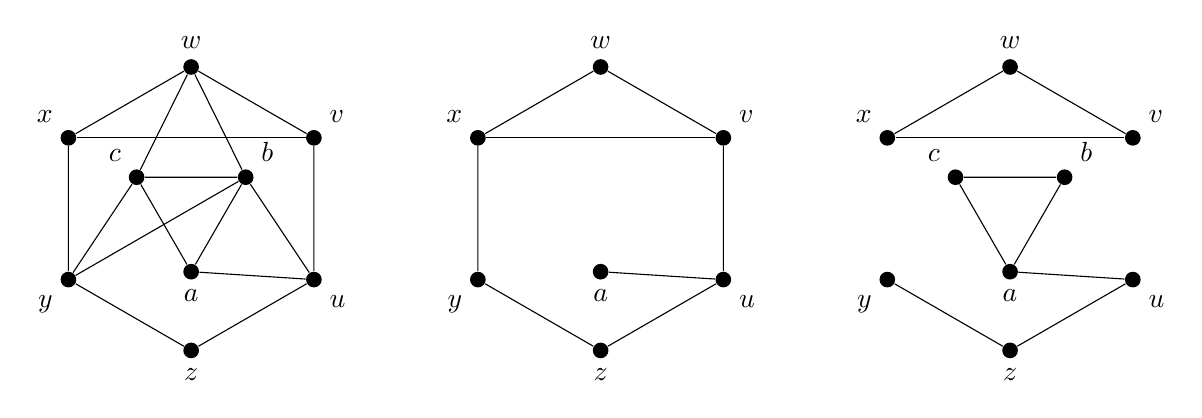
\begin{tikzpicture}[vertex/.style={circle, fill=black, inner sep=2pt}]
    \begin{scope}
      % Outer vertices (on c circle of radius 1.8)
      \node[vertex, label=above:\(w\)]      (w) at (90:1.8)  {};
      \node[vertex, label=above right:\(v\)](v) at (30:1.8)  {};
      \node[vertex, label=below right:\(u\)](u) at (330:1.8) {};
      \node[vertex, label=below:\(z\)]      (z) at (270:1.8) {};
      \node[vertex, label=below left:\(y\)] (y) at (210:1.8) {};
      \node[vertex, label=above left:\(x\)] (x) at (150:1.8) {};
      % Inner vertices (on c circle of radius 0.8)
      \node[vertex, label=above left:\(c\)] (c) at (150:0.8) {};
      \node[vertex, label=below:\(a\)]      (a) at (270:0.8) {};
      \node[vertex, label=above right:\(b\)](b) at (30:0.8)  {};
      % Outer cycle
      \draw (y)--(z)--(u)--(v)--(w)--(x)--(y);
      % Outer diagonal
      \draw (x)--(v);
      % Inner triangle
      \draw (c)--(b)--(a)--(c);
      % Outer-to-inner spokes
      \draw (w)--(c) (w)--(b);
      \draw (y)--(c) (y)--(b);
      \draw (u)--(b) (u)--(b);
      \draw (a)--(u);
    \end{scope}
    % Subgrafo inducido G[{h2,h3,h4,h5}] = K_4
    \begin{scope}[xshift=5.2cm]
      \node[vertex, label=above:\(w\)]      (w) at (90:1.8)  {};
      \node[vertex, label=above right:\(v\)](v) at (30:1.8)  {};
      \node[vertex, label=below right:\(u\)](u) at (330:1.8) {};
      \node[vertex, label=below:\(z\)]      (z) at (270:1.8) {};
      \node[vertex, label=below left:\(y\)] (y) at (210:1.8) {};
      \node[vertex, label=above left:\(x\)] (x) at (150:1.8) {};
      % Inner vertices (on c circle of radius 0.8)
      \node[vertex, label=below:\(a\)]      (a) at (270:0.8) {};
      % Outer cycle
      \draw (y)--(z)--(u)--(v)--(w)--(x)--(y);
      % Outer diagonal
      \draw (x)--(v);
      % Inner triangle
      % Outer-to-inner spokes
      \draw (a)--(u);
    \end{scope}
    % Subgrafo (no inducido): mismos 7 vértices de H, con algunos arcos omitidos
    \begin{scope}[xshift=10.4cm]
      \node[vertex, label=above:\(w\)]      (w) at (90:1.8)  {};
      \node[vertex, label=above right:\(v\)](v) at (30:1.8)  {};
      \node[vertex, label=below right:\(u\)](u) at (330:1.8) {};
      \node[vertex, label=below:\(z\)]      (z) at (270:1.8) {};
      \node[vertex, label=below left:\(y\)] (y) at (210:1.8) {};
      \node[vertex, label=above left:\(x\)] (x) at (150:1.8) {};
      % Inner vertices (on c circle of radius 0.8)
      \node[vertex, label=above left:\(c\)] (c) at (150:0.8) {};
      \node[vertex, label=below:\(a\)]      (a) at (270:0.8) {};
      \node[vertex, label=above right:\(b\)](b) at (30:0.8)  {};
      % Outer cycle
      \draw (y)--(z)--(u);
      \draw (v)--(w)--(x);
      % Outer diagonal
      \draw (x)--(v);
      % Inner triangle
      \draw (c)--(b)--(a)--(c);
      % Outer-to-inner spokes
      \draw (a)--(u);
    \end{scope}
  \end{tikzpicture}
\end{center}

\subsection{Conteo de subgrafos inducidos}
\label{sec:cuantos_subgrafos_inducidos}

Para contar el número de subgrafos inducidos, nótese primero que un subgrafo inducido se genera al remover cualquier selección de \emph{vértices} (lo que elimina solo sus arcos incidentes). No es tan fácil generarlos removiendo arcos, pues se deben mantener las adyacencias.

Con eso en mente, para \hyperref[sec:grafo_completo]{grafo completo} de orden $n$, \(K_n\), existen \(n-1\) subgrafos inducidos módulo isomorfismo, pues quitar un vértice en un grafo completo genera en esencia el mismo grafo que quitar cualquier otro. \(V\) no puede llegar a ser vacío, por lo que se pueden remover \(n-1\) vértices, dando lugar a \(n-1\) subgrafos inducidos módulo isomorfismo.

Ahora, si no se contemplan los isomorfismos entre subgrafos inducidos, para un grafo arbitrario \(G\) (no necesariamente completo), existen exactamente \(2^n-1\) subgrafos inducidos. En este caso, quitar un vértice es diferente a quitar algún otro. Como quitar un vértice genera un subconjunto de \(V\), el número de subgrafos inducidos es el número de subconjuntos de \(V\).

Dicho número de subconjuntos de \(V\) es \(2^n\) por la cardinalidad del conjunto potencia, pues \(|G|=|V|=n\) y \(|\mathcal{P}(V)| = 2^n\). Entre ellos, está el subconjunto vacío, que no constituye un grafo. Substrayéndolo, se obtienen \(2^{n}-1\) subconjuntos no vacíos, cada uno de los cuales representa un subgrafo inducido.

No se conoce una fórmula cerrada para contar los subgrafos inducidos módulo isomorfismo de un grafo no completo.

%TODO: No hay una fórmula fácil para el número de subgrafos, es una sumatoria fea, pero podría añadirse esa sección.
% \subsubsection{¿Cuántos subgrafos?}
% \label{sec:cuantos_subgrafos}
